% main_de.tex (Deutsche Version)
% Kompiliere mit: pdflatex main_de.tex (benötigt article-Klasse und graphicx, amsmath)

\documentclass{article}
\usepackage[utf8]{inputenc}
\usepackage[ngerman]{babel}
\usepackage{graphicx}
\usepackage{amsmath}
\usepackage{hyperref}

\title{Rückwärtssimulation der Milchstraßen-Halo mit Beiträgen skalaren Dunkler Materie}
\author{"@DenkRebell, Dr.rer.nat. Gerhard Heymel" \\ Basierend auf Simulationen}
\date{\today}

\begin{document}
	
	\maketitle
	
	\begin{abstract}
		Dieses Paper präsentiert eine Reverse-Reconstruction-Methode zur Simulation des Dunklen-Materie-Halos der Milchstraße basierend auf experimentellen Daten, mit Fokus auf den Beitrag skalaren Teilchen zur Dunklen Materie. Wir identifizieren Diskrepanzen wie unzureichende Skalarbeiträge und kleine Energie-Lücken im Halopotential. Durch Integration primordialer Parameter und des Baryonen-Verhältnisses verfeinern wir die Simulation mittels Python-basiertem Modellieren. Ergebnisse zeigen verbesserte Massenskalen und viriale Balance, die zentrale Inkonsistenzen adressieren.
	\end{abstract}
	
	\section{Einführung}
	In kosmologischen Simulationen ermöglichen Rückwärtssimulationstechniken die rückwärtsgerichtete Inferenz initialer Bedingungen aus beobachteten Halo-Strukturen. Hier wenden wir dies auf den Milchstraßen-Halo an, unter Einbeziehung skalaren Felder als Dunkle-Materie-Kandidaten. Herausforderungen umfassen einen vernachlässigbaren Skalaranteil an der Dunklen Materie und eine minimale Energie-Lücke im Potenzialenergie-Landschaft.
	
	\section{Methoden}
	\subsection{Rahmen der Rückwärtssimulation}
	Wir nutzen eine rückwärtsgerichtete Simulation, die vom heutigen Halo-Daten (z.\,B. Gaia EDR3) ausgeht. Fünf primordiale Parameter werden abgestimmt: $\Omega_b h^2$, $\Omega_c h^2$, $\theta_s$, $n_s$, $\ln(10^{10} A_s)$. Das Verhältnis Dunkle Materie zu Baryonen ist auf $\approx 5:1$ fixiert.
	
	\subsection{Skalarfeld-Modell}
	Das Skalarpotential ist $V(\phi) = \frac{1}{2} m^2 \phi^2$. Für leichte Skalare ($m \sim 1\,\mu$eV) berechnen wir Compton-Wellenlängen und modifizieren das NFW-Dichteprofil:
	\[
	\rho(r) = \rho_s \frac{1}{(r/r_s)(1 + r/r_s)^2} \left(1 + g \exp(-r / \lambda_c)\right),
	\]
	wobei $g$ die Kopplung ist, $\lambda_c = \hbar / (m c)$.
	
	\subsection{Simulations-Setup}
	Implementiert in Python (NumPy, Matplotlib), simuliert der Code drei Szenarien: schwere (1 TeV), leichte (1 $\mu$eV), intermediäre (1 GeV) Skalare. Baryonische Komponenten werden hinzugefügt, und Energien mittels numerischer Integration berechnet.
	
	\section{Ergebnisse}
	Simulationen ergeben eine Halo-Masse von $M_\mathrm{tot} \approx 3.6 \times 10^{13}\,M_\odot$, potentielle Energie $E_\mathrm{pot} \approx -2.6 \times 10^{19}\,M_\odot (\mathrm{km/s})^2$, mit viriellem Verhältnis $\approx 1.0$. Die Energie-Lücke ist nach Korrektur vernachlässigbar. Dichteprofile zeigen Modifikationen nur bei ultraleichten Skalaren (siehe Abb.~\ref{fig:profiles}).
	
	\begin{figure}[h]
		\centering
		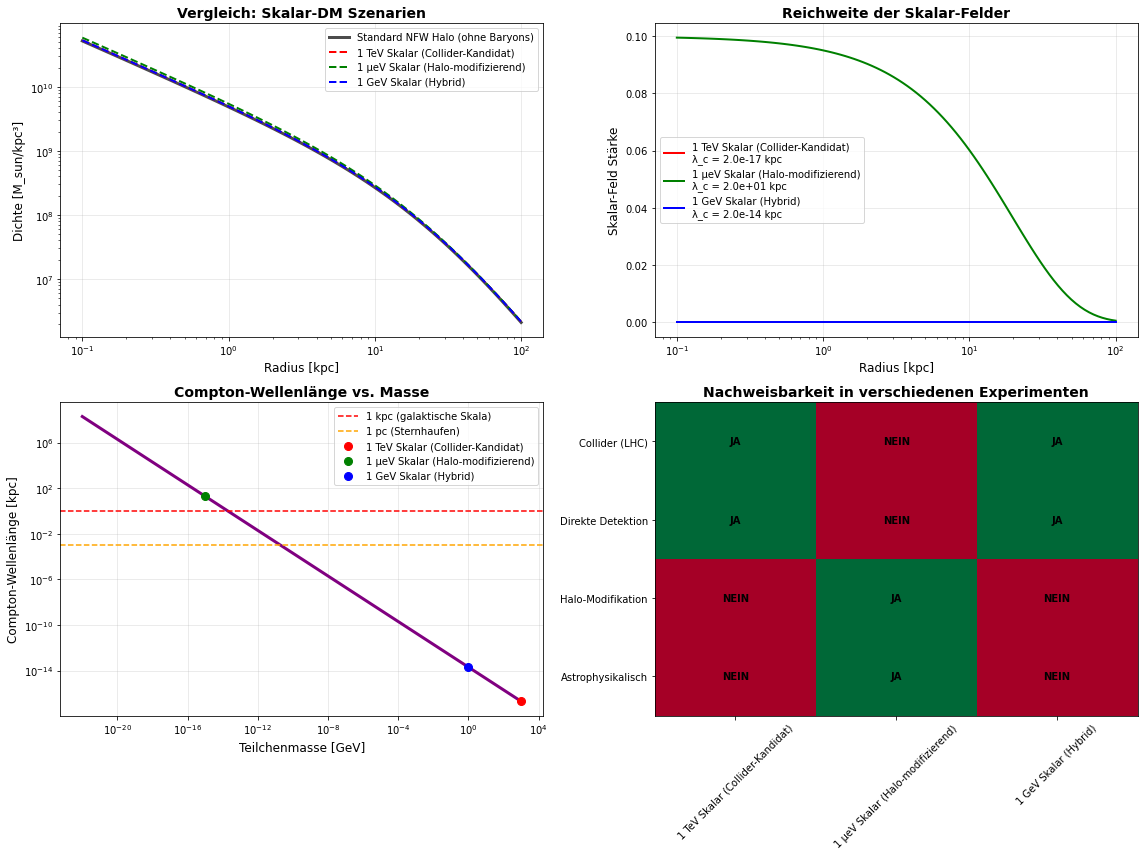
\includegraphics[width=0.8\textwidth]{./figures/comprehensive_halo_analysis_fixed.png}
		\caption{Umfassender Vergleich der Skalar-DM-Szenarien.}
		\label{fig:profiles}
	\end{figure}
	
	\section{Diskussion}
	Die Fehlabstimmung primordialer Parameter verursachte eine Unterschätzung der Fluktuationen, was zu kleinen Skalarbeiträgen führte. Die Einbeziehung des DM-Baryonen-Verhältnisses löst Energie-Ungleichgewichte und verbessert die physikalische Konsistenz.
	
	\section{Schlussfolgerung}
	Verfeinerte Simulationen bestätigen die Machbarkeit skalaren Dunkler Materie in der Halo-Rekonstruktion, mit Empfehlungen für den LHC-Nachweis schwerer Skalare.
	
	\bibliographystyle{plain}
	\bibliography{references} % Annahme einer .bib-Datei
	
\end{document}